\section{General sewer construction}\label{se:sewer_construction}
Furthermore an illustration of the process wastewater undergoes from it is used at the consumer to it is treated at the plant will be explained. 

In figure \ref{fig:sewer_overview_of_the_different_parts} a block diagram of the process wastewater undergoes is illustrated.
\begin{figure}[H]
\centering
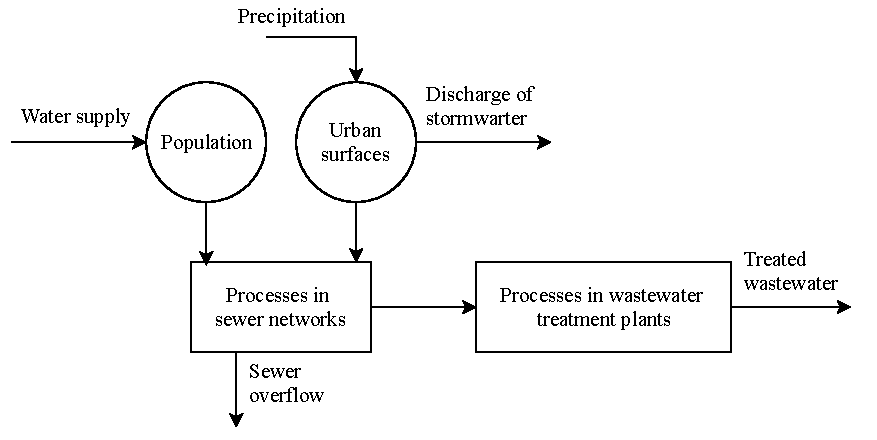
\includegraphics[width=1\textwidth]{report/introduction/pictures/sewer_process2.pdf}
\caption{Arbejdsblad billede, inspiration er taget fra hvitved.}
\label{fig:sewer_overview_of_the_different_parts}
\end{figure}
From the left the precipitation over urban surfaces are collected in the sewers. If the precipitation are to much for the sewer to handle it will be discharged in a storm water sewer, which will lead the water into small rivers or be collected in tanks \fxnote{Skriv hvad det bliver brugt til}. Furthermore from the left the water supplies goes into the consumers of the water, such as the industry or households. These will produce wastewater that is lead into the sewers. Within the sewers chemical and microbial reactions occurs, which will be explained in section \ref{subse:chemical_reactions_in_a_sewer}. If the sewer is overfilled the sewage is lead into rivers and fields to prevent flooding in households, industry and on the urban surfaces. The sewer leads the wastewater to the wastewater treatment plant, where the wastewater will be filtered before sending it back into the environment, which will be explained in greater detail in section \ref{subse:Wastewater treatment plant}. 

Typically the water treatment plant are constructed near rivers or fjord which is typical at a lower geographical location, thereby enabling the force of the gravity to transport the wastewater in a sewer. If the industry or the households are at a lower geographical location than the water treatment plant, then pumps are used to transport the wastewater as illustrated in figure \ref{fig:Sewer_drawing}.
\begin{figure}[H]
\centering
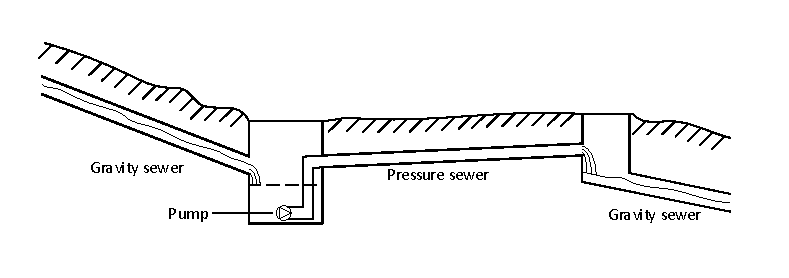
\includegraphics[width=1\textwidth]{report/introduction/pictures/Sewer_drawing.pdf}
\caption{Illustrate different methods for transportation of wastewater.}
\label{fig:Sewer_drawing}
\end{figure}

The pipes are often constructed in concrete or polyethylene. Where concrete pipes are used for gravity sewers and polyethylene are used in a pressure sewer due to a lower roughness height which means less friction from the surface of the pipe. 